% !TeX root = ../main.tex

\paragraph{Homework \#3 Crystal lattice}

\begin{problem}[Crystallographic restriction theorem]
  Proof the crystallographic restriction theorem: Consider a crystal (i.e. with
  translational symmetry) in three dimensions that is invariant under rotations
  by an angle $2\pi/n$ around an axis. Then the only allowed possibilities are
  $n = 1$, $2$, $3$, $4$, $6$ with the case $n = 1$ being the trivial case
  with no rotational symmetry.
\end{problem}
\begin{solution}\begin{proof}
  When taking the rotation matrix to an arbitary vector
  $\bm l = (l_1, l_2, l_3)\tran$, it should leave the lattice invariant,
  the trace of the rotation matrix
  \[
    \mathbf R = \begin{pmatrix}
      \cos\theta & -\sin\theta & 0\\
      \sin\theta & \cos\theta & 0\\
      0 & 0 & 1
    \end{pmatrix}
  \]
  must be integers, then $\Tr(\mathbf R) \in \mathbb Z$,
  $n \in \{1,2,3,4,6\}$.
\end{proof}
\end{solution}

\begin{wrapstuff}[r, width = .24\linewidth]
  \centering
  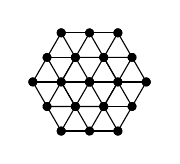
\begin{tikzpicture}[scale = .36]
    \foreach \i in {0, 1, 2, 3, 4, 5} {
      \foreach \j in {0, 1, 2} {
        \draw [rotate around = {-\i * 60:(0,0)}]
          ({-2 + \j/2}, {sqrt(3)*\j/2}) --++ (2,0);
          \foreach \k in {0, 1, 2}
            \fill [rotate around = {-\i * 60:(0,0)}]
              ({-\j + \k/2}, {sqrt(3)*\k/2}) circle (.16);
      }
      \draw [rotate around = {-\i * 60:(0,0)}] (-1,0) --++ (1,{sqrt(3)});
    }
  \end{tikzpicture}
\end{wrapstuff}
\begin{problem}[2D triangular lattice]
  Let us consider a two-dimen\-sional triangular lattice as shown in the
  following figure.
  \wrapstuffclear
  \begin{enumext}
    \item Identify the primitive unit cell of the two-dimensional triangular
    lattice. Find the basis vectors.
    \item Construct the basis vectors of the reciprocal unit cell.
  \end{enumext}
\end{problem}
\begin{solution}\leavevmode
  \begin{enumext}
    \item $\bm a_1 = a(1,0)$, $\bm a_2 = a \ab(\frac12, \frac{\sqrt3}{2})$.
    \item Using the relation $\bm a_i \cdot \bm b_j = 2\pi\delta_{ij}$ for
    $\bm a_{1,2}$ and $\bm b_{1,2}$, then
    $\bm b_1 = \frac{2\pi}a \ab(1, -\frac1{\sqrt3})$,
    $\bm b_2 = \frac{2\pi}a \ab(0, \frac2{\sqrt3})$.
  \end{enumext}
\end{solution}

\begin{problem}[Properties of the reciprocal lattice]\leavevmode
  \begin{enumext}
    \item Show that all reciprocal lattice vectors of the form
    $\bm G = h\bm A + k\bm B + l\bm C$ are perpendicular to the planes of the
    same indices $(h, k, l)$ in real space.
    \item Show that the distance $d_{h,k,l}$ between two consecutive planes
    $(h, k, l)$ is inversely proportional to $|\bm G_{h,k,l}|$.
    \item Find $d_{h,k,l}$ for a simple cubic lattice and an orthorhombic
    lattice ($a \neq b \neq c$, $\alpha = \beta = \gamma = \pi/2$).
  \end{enumext}
\end{problem}
\begin{solution}\leavevmode
  \begin{enumext}
    \item
    \begin{proof}
      Express $\bm G$ in terms of the reciprocal lattice vectors
      \[
        \bm G = \frac{2\pi}{\bm a_1 \cdot (\bm a_2 \times \bm a_3)}
           [h(\bm a_2 \times \bm a_3) + k(\bm a_3 \times \bm a_1)
          + l(\bm a_1 \times \bm a_2)]
      \]
      with the Miller indices $h:k:l = \frac1{a_1}:\frac1{a_2}:\frac1{a_3}$.
      In real space, the normal vector of the plane $(h, k, l)$ can be
      expressed as\\
      \begin{minipage}{.64\linewidth}
        \[
          \begin{aligned}
            \hat{\bm n}_{hkl} & \sim \bm r_1 \times \bm r_2
          = \frac1{hkl} [h(\bm a_2 \times \bm a_3) \\
        & \quad + k(\bm a_3 \times \bm a_1) +
                  l(\bm a_1 \times \bm a_2)],\\
          \bm r_1 & = \vec{DE} = \bm a_2/k - \bm a_1/h,\\
          \bm r_2 & = \vec{EF} = \bm a_3/l - \bm a_2/k.
          \end{aligned}
        \]
      \end{minipage}
      \hfill
      \begin{minipage}{.32\linewidth}
        \centering
        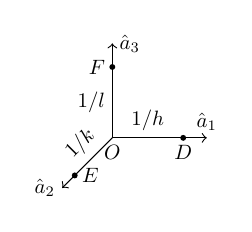
\begin{tikzpicture}[scale = .75, every node/.style = {scale = .75}]
          \draw [->] (0,0) -- (1.6,0) node [above] {$\hat a_1$};
          \draw [->] (0,0) -- (0,1.6) node [right] {$\hat a_3$};
          \draw [->] (0,0) -- (-135:1.2) node [left] {$\hat a_2$};
          \fill (1.2,0) circle (.05) node [below] {$D$};
          \node [above] at (.6,0) {$1/h$};
          \fill (0,1.2) circle (.05) node [left] {$F$};
          \node [left] at (0,.6) {$1/l$};
          \fill (-135:.9) circle (.05) node [right] {$E$};
          \node [above left, inner sep = -3pt] at
            (-135:.45) {\rotatebox{45}{$1/k$}};
          \node [below] at (0,0) {$O$};
        \end{tikzpicture}
      \end{minipage}
      Hence, $\hat{\bm n}_{hkl} \parallel \bm G$, so $\bm G$ is perpendicular
      to $(h, k, l)$ plane.
    \end{proof}
    \item \begin{proof}
    The vectors pointing to the $n + 1$ and $n$-th plane satisfy
    \[
      \bm G \cdot \bm d_{n+1} = 2\pi(n + 1), \qq{and}
      \bm G \cdot \bm d_n = 2\pi n,
    \]
    where $\bm d_{n+1} - \bm d_n = d \hat{\bm n}$. Combine the two relations
    \[
      \bm G \cdot(\bm r_{n+1} - \bm r_n) = \bm G \cdot \bm{\hat n} d = 2\pi d.
    \]
    So, we proved $d = 2\pi/(\bm G_{h,k,l} \cdot \bm{\hat n})
    = 2\pi/|\bm G_{h,k,l}|$.
    \end{proof}
    \item For a simple cubic lattice
    \[
      \bm a = (a,0,0), \quad \bm b = (0,b,0), \quad \bm c = (0,0,c).
    \]
    Then, the reciprocal vectors can be expressed as
    \[
      \bm G = \frac{2\pi h}{a} \bm{\hat x} +
              \frac{2\pi k}{b} \bm{\hat y} +
              \frac{2\pi l}{c} \bm{\hat z}.
    \]
    So, we obtain the distance $d = \frac{2\pi}{|\bm G|}
    = \ab(\frac{h^2}{a^2} + \frac{k^2}{b^2} + \frac{l^2}{c^2})^{-1/2}$.
  \end{enumext}
\end{solution}

\begin{problem}[Atomic planes and Miller indices: application to lithium]
  The Bravais lattice of lithium is simple cubic with lattice parameter
  $a = \qty{3.48}\angstrom$.
  \begin{enumext}
    \item Suppose that the atoms (assumed to be spheres) are placed along the
    $[111]$, represent the atomic distribution along the following faces
    $(100)$, $(110)$, $(111)$, and $(201)$.
    \item For each such 2D structure, state the direction and basis vector,
    $\bm a$ and $\bm b$ of the elementary lattice as well as the value of the
    angle, $\gamma$.
    \item Find the atomic concentration and the mass density of lithium
    ($A \approx 7$).
  \end{enumext}
\end{problem}
\begin{solution}\leavevmode
  \begin{enumext}
    \item (b)
    \begin{enumext}
      \item [$(100)$] $\bm a = (0,a,0)$, $\bm b = (0,0,a)$,
      $\gamma = \braket<a,b> = \qty{90}\degree$.
      \item [$(110)$] $\bm a = (a,-a,0)$, $\bm b = (0,0,a)$,
      $\gamma = \braket<a,b> = \qty{90}\degree$.
      \item [$(111)$] $\bm a = (a,0,-a)$, $\bm b = (0,a,a)$,
      $\gamma = \braket<a,b> = \qty{60}\degree$.
      \item [$(201)$] $\bm a = (0,a,0)$, $\bm b = (a,0,-2a)$,
      $\gamma = \braket<a,b> = \qty{90}\degree$.
    \end{enumext}
    \addtocounter{enumXi}{1}
    \item Since the atoms are placed along the $[111]$, then every cubic
    lattice's corners has an atom, i.e., it is equivalent that there is an
    atom in every lattice. So, the atomic concentration is
    \[
      n = \frac1V = \frac1{a^3} = \qty{2.3728e28}{atoms/\m^3}.
    \]
    The mass density is
    \[
      \rho = n m_\text{atom} = nA/N_A = \qty{275.816}{\kg/\m^3}.
    \]
  \end{enumext}
\end{solution}